\documentclass{standalone}
\usepackage{tikz}
\usetikzlibrary{patterns, positioning}

\begin{document}
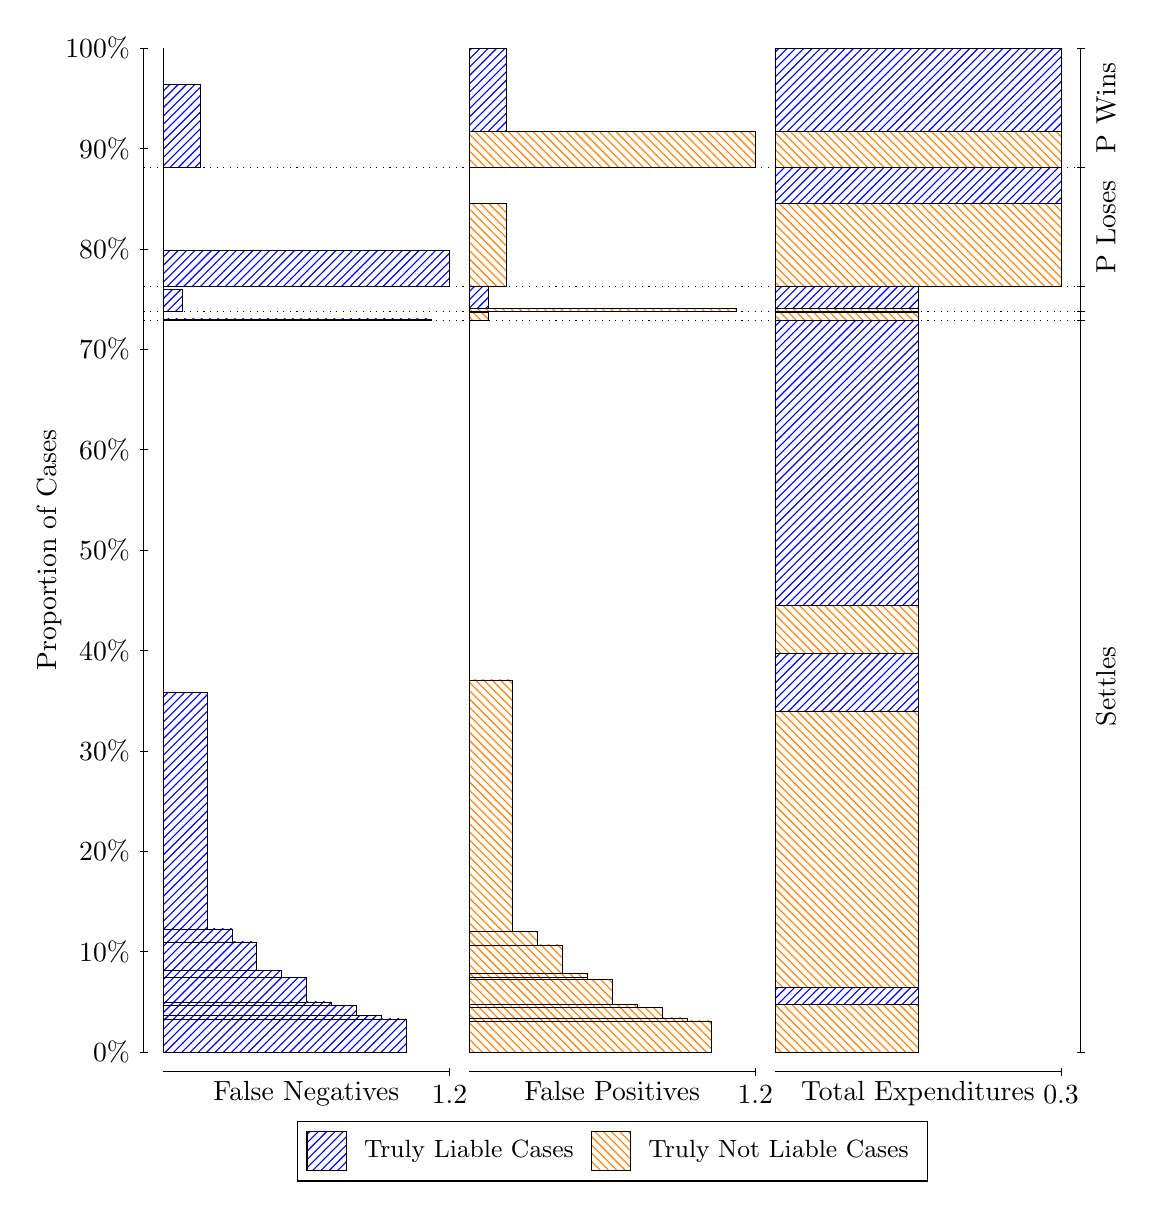
\begin{tikzpicture}
\draw[black, very thin] (1.5,1.75) -- (1.5,14.5);
\node[rotate=90, anchor=center] at (0.3, 8.125) {Proportion of Cases};
\draw[black, very thin] (1.45,1.75) -- (1.55,1.75);
\node[anchor=east] at (1.45, 1.75) {0\%};
\draw[black, very thin] (1.45,3.025) -- (1.55,3.025);
\node[anchor=east] at (1.45, 3.025) {10\%};
\draw[black, very thin] (1.45,4.3) -- (1.55,4.3);
\node[anchor=east] at (1.45, 4.3) {20\%};
\draw[black, very thin] (1.45,5.575) -- (1.55,5.575);
\node[anchor=east] at (1.45, 5.575) {30\%};
\draw[black, very thin] (1.45,6.85) -- (1.55,6.85);
\node[anchor=east] at (1.45, 6.85) {40\%};
\draw[black, very thin] (1.45,8.125) -- (1.55,8.125);
\node[anchor=east] at (1.45, 8.125) {50\%};
\draw[black, very thin] (1.45,9.4) -- (1.55,9.4);
\node[anchor=east] at (1.45, 9.4) {60\%};
\draw[black, very thin] (1.45,10.675) -- (1.55,10.675);
\node[anchor=east] at (1.45, 10.675) {70\%};
\draw[black, very thin] (1.45,11.95) -- (1.55,11.95);
\node[anchor=east] at (1.45, 11.95) {80\%};
\draw[black, very thin] (1.45,13.225) -- (1.55,13.225);
\node[anchor=east] at (1.45, 13.225) {90\%};
\draw[black, very thin] (1.45,14.5) -- (1.55,14.5);
\node[anchor=east] at (1.45, 14.5) {100\%};

\draw[black, very thin] (13.4,1.75) -- (13.4,14.5);
\draw[black, very thin] (13.35,1.75) -- (13.45,1.75);
\node[anchor=west] at (13.35, 1.75) {};
\draw[black, very thin] (13.35,11.038) -- (13.45,11.038);
\node[anchor=west] at (13.35, 11.038) {};
\draw[black, very thin] (13.35,11.159) -- (13.45,11.159);
\node[anchor=west] at (13.35, 11.159) {};
\draw[black, very thin] (13.35,11.47) -- (13.45,11.47);
\node[anchor=west] at (13.35, 11.47) {};
\draw[black, very thin] (13.35,12.983) -- (13.45,12.983);
\node[anchor=west] at (13.35, 12.983) {};
\draw[black, very thin] (13.35,14.5) -- (13.45,14.5);
\node[anchor=west] at (13.35, 14.5) {};

\draw[black, very thin, pattern color=blue, pattern=north east lines] (1.75,1.75) rectangle (4.8304,2.1714);
\draw[black, very thin, pattern color=blue, pattern=north east lines] (1.75,2.1714) rectangle (4.5145,2.2119);
\draw[black, very thin, pattern color=blue, pattern=north east lines] (1.75,2.2119) rectangle (4.1986,2.3428);
\draw[black, very thin, pattern color=blue, pattern=north east lines] (1.75,2.3428) rectangle (3.8826,2.3866);
\draw[black, very thin, pattern color=blue, pattern=north east lines] (1.75,2.3866) rectangle (3.5667,2.6987);
\draw[black, very thin, pattern color=blue, pattern=north east lines] (1.75,2.6987) rectangle (3.2507,2.783);
\draw[black, very thin, pattern color=blue, pattern=north east lines] (1.75,2.783) rectangle (2.9348,3.1493);
\draw[black, very thin, pattern color=blue, pattern=north east lines] (1.75,3.1493) rectangle (2.6188,3.3145);
\draw[black, very thin, pattern color=blue, pattern=north east lines] (1.75,3.3145) rectangle (2.3029,6.3132);
\draw[black, very thin, pattern color=orange, pattern=north west lines] (1.75,6.3132) rectangle (1.75,11.038);
\draw[black, very thin, pattern color=blue, pattern=north east lines] (1.75,11.038) rectangle (5.1464,11.059);
\draw[black, very thin, pattern color=orange, pattern=north west lines] (1.75,11.059) rectangle (1.75,11.159);
\draw[black, very thin, pattern color=blue, pattern=north east lines] (1.75,11.159) rectangle (1.987,11.433);
\draw[black, very thin, pattern color=orange, pattern=north west lines] (1.75,11.433) rectangle (1.75,11.47);
\draw[black, very thin, pattern color=blue, pattern=north east lines] (1.75,11.47) rectangle (5.3833,11.93);
\draw[black, very thin, pattern color=orange, pattern=north west lines] (1.75,11.93) rectangle (1.75,12.983);
\draw[black, very thin, pattern color=blue, pattern=north east lines] (1.75,12.983) rectangle (2.2239,14.04);
\draw[black, very thin, pattern color=orange, pattern=north west lines] (1.75,14.04) rectangle (1.75,14.5);
\draw[black, very thin, pattern color=orange, pattern=north west lines] (5.6333,1.75) rectangle (8.7138,2.1453);
\draw[black, very thin, pattern color=orange, pattern=north west lines] (5.6333,2.1453) rectangle (8.3978,2.1839);
\draw[black, very thin, pattern color=orange, pattern=north west lines] (5.6333,2.1839) rectangle (8.0819,2.3157);
\draw[black, very thin, pattern color=orange, pattern=north west lines] (5.6333,2.3157) rectangle (7.7659,2.3586);
\draw[black, very thin, pattern color=orange, pattern=north west lines] (5.6333,2.3586) rectangle (7.45,2.6696);
\draw[black, very thin, pattern color=orange, pattern=north west lines] (5.6333,2.6696) rectangle (7.1341,2.6925);
\draw[black, very thin, pattern color=orange, pattern=north west lines] (5.6333,2.6925) rectangle (7.1341,2.7496);
\draw[black, very thin, pattern color=orange, pattern=north west lines] (5.6333,2.7496) rectangle (6.8181,3.1114);
\draw[black, very thin, pattern color=orange, pattern=north west lines] (5.6333,3.1114) rectangle (6.5022,3.2784);
\draw[black, very thin, pattern color=orange, pattern=north west lines] (5.6333,3.2784) rectangle (6.1862,6.4749);
\draw[black, very thin, pattern color=blue, pattern=north east lines] (5.6333,6.4749) rectangle (5.6333,11.038);
\draw[black, very thin, pattern color=orange, pattern=north west lines] (5.6333,11.038) rectangle (5.8703,11.138);
\draw[black, very thin, pattern color=blue, pattern=north east lines] (5.6333,11.138) rectangle (5.6333,11.159);
\draw[black, very thin, pattern color=orange, pattern=north west lines] (5.6333,11.159) rectangle (9.0297,11.196);
\draw[black, very thin, pattern color=blue, pattern=north east lines] (5.6333,11.196) rectangle (5.8703,11.47);
\draw[black, very thin, pattern color=orange, pattern=north west lines] (5.6333,11.47) rectangle (6.1072,12.523);
\draw[black, very thin, pattern color=blue, pattern=north east lines] (5.6333,12.523) rectangle (5.6333,12.983);
\draw[black, very thin, pattern color=orange, pattern=north west lines] (5.6333,12.983) rectangle (9.2667,13.443);
\draw[black, very thin, pattern color=blue, pattern=north east lines] (5.6333,13.443) rectangle (6.1072,14.5);
\draw[black, very thin, pattern color=orange, pattern=north west lines] (9.5167,1.75) rectangle (11.333,2.3588);
\draw[black, very thin, pattern color=blue, pattern=north east lines] (9.5167,2.3588) rectangle (11.333,2.5739);
\draw[black, very thin, pattern color=orange, pattern=north west lines] (9.5167,2.5739) rectangle (11.333,6.0814);
\draw[black, very thin, pattern color=blue, pattern=north east lines] (9.5167,6.0814) rectangle (11.333,6.8151);
\draw[black, very thin, pattern color=orange, pattern=north west lines] (9.5167,6.8151) rectangle (11.333,7.4237);
\draw[black, very thin, pattern color=blue, pattern=north east lines] (9.5167,7.4237) rectangle (11.333,11.038);
\draw[black, very thin, pattern color=orange, pattern=north west lines] (9.5167,11.038) rectangle (11.333,11.138);
\draw[black, very thin, pattern color=blue, pattern=north east lines] (9.5167,11.138) rectangle (11.333,11.159);
\draw[black, very thin, pattern color=orange, pattern=north west lines] (9.5167,11.159) rectangle (11.333,11.196);
\draw[black, very thin, pattern color=blue, pattern=north east lines] (9.5167,11.196) rectangle (11.333,11.47);
\draw[black, very thin, pattern color=orange, pattern=north west lines] (9.5167,11.47) rectangle (13.15,12.523);
\draw[black, very thin, pattern color=blue, pattern=north east lines] (9.5167,12.523) rectangle (13.15,12.983);
\draw[black, very thin, pattern color=orange, pattern=north west lines] (9.5167,12.983) rectangle (13.15,13.443);
\draw[black, very thin, pattern color=blue, pattern=north east lines] (9.5167,13.443) rectangle (13.15,14.5);
\draw[black, dotted] (1.5,11.038) -- (13.4,11.038);
\draw[black, dotted] (1.5,11.159) -- (13.4,11.159);
\draw[black, dotted] (1.5,11.47) -- (13.4,11.47);
\draw[black, dotted] (1.5,12.983) -- (13.4,12.983);
\draw[black, very thin] (1.75,1.5) -- (5.3833,1.5);
\node[anchor=north] at (3.5667, 1.5) {False Negatives};
\draw[black, very thin] (5.3833,1.45) -- (5.3833,1.55);
\node[anchor=north] at (5.3833, 1.45) {1.2};

\draw[black, very thin] (5.6333,1.5) -- (9.2667,1.5);
\node[anchor=north] at (7.45, 1.5) {False Positives};
\draw[black, very thin] (9.2667,1.45) -- (9.2667,1.55);
\node[anchor=north] at (9.2667, 1.45) {1.2};

\draw[black, very thin] (9.5167,1.5) -- (13.15,1.5);
\node[anchor=north] at (11.333, 1.5) {Total Expenditures};
\draw[black, very thin] (13.15,1.45) -- (13.15,1.55);
\node[anchor=north] at (13.15, 1.45) {0.3};

\node[black, centered, rotate=90] at (13.72, 6.394) {Settles};


\node[black, centered, rotate=90] at (13.72, 12.226) {P Loses};
\node[black, centered, rotate=90] at (13.72, 13.741) {P Wins};

\draw (7.449999999999999,1.5) node[draw=none] (baseCoordinate) {};
\begin{scope}[align=center]
        \matrix[scale=0.5, draw=black, below=0.5cm of baseCoordinate, nodes={draw}, column sep=0.1cm]{
            \node[rectangle, draw, minimum width=0.5cm, minimum height=0.5cm, pattern=north east lines, pattern color=blue] {}; &
            \node[draw=none, font=\small] (B) {Truly Liable Cases}; &
            \node[rectangle, draw, minimum width=0.5cm, minimum height=0.5cm, pattern=north west lines, pattern color=orange] {}; &
            \node[draw=none, font=\small] (B) {Truly Not Liable Cases}; \\
            };
\end{scope}

\end{tikzpicture}
\end{document}